\documentclass[11pt]{article}
\usepackage[utf8]{inputenc}
%\usepackage[latin1]{inputenc}
\usepackage[spanish]{babel}
\usepackage{anysize}
\usepackage{graphicx}
\usepackage{siunitx}
\usepackage{amsmath}
\usepackage[outdir=./]{epstopdf}
\usepackage{tikz}
\usepackage{circuitikz}
\usepackage{float}
\usepackage{standalone}
\renewcommand{\baselinestretch}{1.2}
\spanishdecimal{.} 
\marginsize{1.5cm}{1.5cm}{0cm}{2cm}  
\title{Examen Reposición Primer Parcial \\ Curso de Física Computacional}
\author{M. en C. Gustavo Contreras Mayén}
\date{ }
\begin{document}
\maketitle
\fontsize{14}{14}\selectfont
\begin{enumerate}
\item Identifica los números de punto flotante correspondientes a las siguientes cadenas de bits (debes de resolverlo mediante un código, para simplificar la tarea, considera una conversión de binario a decimal simple, es decir, no uses el estándar IEEE)
\begin{enumerate}
\item \fbox{0 \hspace{0.1cm} 00000000 \hspace{0.1cm} 00000000000000000000000}
\item \fbox{1 \hspace{0.1cm} 00000000 \hspace{0.1cm} 00000000000000000000000}
\item \fbox{0 \hspace{0.1cm} 11111111 \hspace{0.1cm} 00000000000000000000000}
\item \fbox{1 \hspace{0.1cm} 11111111 \hspace{0.1cm} 00000000000000000000000}
\item \fbox{0 \hspace{0.1cm} 00000001 \hspace{0.1cm} 00000000000000000000000}
\item \fbox{0 \hspace{0.1cm} 10000001 \hspace{0.1cm} 01100000000000000000000}
\item \fbox{0 \hspace{0.1cm} 01111111 \hspace{0.1cm} 00000000000000000000000}
\item \fbox{0 \hspace{0.1cm} 01111011 \hspace{0.1cm} 10011001100110011001100}
\end{enumerate}
\item Da la representación en binario con precisión simple de los siguientes números decimales
\begin{enumerate}
\item -9876.54321
\item 0.2343375
\item -285.75
\item $10^{2}$
\item $+0.0$ y $-0.0$
\end{enumerate}
\item La función gamma $\Gamma (x)$, se define como la siguiente integral
\[ \Gamma (x) = \int_{0}^{\infty} t^{x-1} \: e^{-t} dt\]
que converge para todo $x$ positivo, pese a que para $0<x<1$ el integrando tiene una divergencia en $t=0$.
\par
Calcula numéricamente a partir de la definción anterior, la $\Gamma$ para $x = 10$ y $x = 1/2$, valores para los cuales se conocen los resultados analíticos:
\begin{align*}
\Gamma(10) &= 9! = 362880 \\
\Gamma(1/2) &= \sqrt{\pi}
\end{align*}
En cada caso debes:
\begin{enumerate}
\item indicar el cambio de variable utilizado.
\item el número de puntos utilizados en la discretización.
\item el método de integración.
\item el resultado obtenido.
\item el error cometido respecto al valor analítico, usando las funciones de \texttt{scipy}.
\end{enumerate}
\item Evalúa numéricamente las siguientes integrales:
\begin{align*}
I_{1} &= \int_{0}^{\infty} e^{-x} \:  ln \; x \: dx \\
I_{2} &= \int_{0}^{1} \dfrac{1+x}{1-x^{3}} \: ln\dfrac{1}{x} dx
\end{align*}
El problema consiste en resolver las integrales con algún cambio de variable para tener un integrando suave en un intervalo finito.
\par
Se debe de obtener un resultado razonablemente bueno, teniendo que evaluar el integrando final con el menor número ($N$) de veces que sea posible. Como criterio de convergencia debes de usar alguna cantidad como
\[ \epsilon = \dfrac{I - I_{N}}{I} < 10^{-n}\]
con n = $2,3,4,5,6$
En cada caso debes:
\begin{enumerate}
\item indicar el(los) cambio(s) de variable utilizado(s).
\item el número de puntos utilizados en la discretización.
\item el método de integración.
\item el resultado obtenido.
\item el error cometido respecto al valor de I.
\end{enumerate}
\item La posición de equilibrio de un cilindro flotante es $h = r$. Si el cilindro se desplaza a la posición $h = 1.5 \: r$ y se libera, la ecuación diferencial que describe el movimiento es
\[ \ddot{y} = \dfrac{2}{\pi} \: \left[ \tan^{-1} \: \dfrac{1 - y}{\sqrt{2 \: y - y^{2}}} + (1 - y) \: \sqrt{2 \: y - y^{2}} \right] \]
donde $y = h / r$.
\begin{figure}[H]
\centering
\begin{tikzpicture}
	\node[circle, draw, minimum size=4cm] (A) at  (0,0) {};
	\draw [dash pattern={on 7pt off 2pt on 1pt off 3pt}] (-2.5, 0) -- (2.5, 0);
	\draw [dash pattern={on 7pt off 2pt on 1pt off 3pt}] (0, -2.5) -- (0, 2.5);
	\draw [arrows=->, thick] (0,0) -- ++(45:2) node [midway, above] {$r$};
	\draw (0, -2) -- (3.5, -2);
	\draw [arrows=->, thick, color=white] (0,0) -- ++(210:2) coordinate (B);
	\draw [arrows=->, thick, color=white] (0,0) -- ++(-30:2) coordinate (C);
	\draw (-4, -1) -- (B);
	\draw [dash pattern=on 3pt off 2pt] (B) -- (C);
	\draw (C) -- (3.5, -1);
	\draw [arrows=<->] (3.2, -1) -- (3.2, -2) node [midway, left] {$h$};
	\draw (-4, 0.25) node {Nivel del agua};
	\draw [arrows=->] (-3.7, 0.1	) -- (-3.5, -1);
\end{tikzpicture}
\end{figure}
Grafica $h/r$ desde $t = 0$ hasta $t = 6$. A partir de la gráfica estima el período del movimiento resultante.
\item Las leyes de Kirchoff para el siguiente circuito son
\begin{align}
L \: \dfrac{d i_{1}}{dt} +  R \: i_{1} + 2 \: R (i_{1} + i_{2}) &=  E(t) \label{eq:ecuacion_a} \\
\dfrac{q_{2}}{C} + R \: i_{2} + 2 \: R \: (i_{2} + i_{1}) &= E(t) \label{eq:ecuacion_b}
\end{align}
\begin{figure}[H]
	\centering
	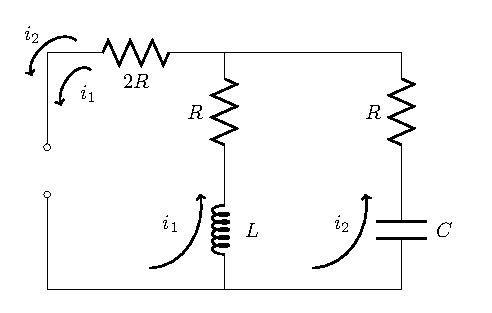
\includegraphics[scale=1.3]{Figuras/circuito_reposicion_01.eps}
	\caption{Circuito RLC en paralelo para el ejercicio.}
\end{figure}
Donde $i_{1}$ e $i_{2}$ son las corrientes dentro de las mallas, $q_{2}$ es la carga en el condensador.
\par
Diferenciando la ecuación (\ref{eq:ecuacion_b}) y sustituyendo la relación carga-corriente $d q_{2}/ dt = i_{2}$, se obtiene
\begin{align}
\dfrac{d i_{1}}{dt} &= \dfrac{-3 \: R \: i_{1} - 2 \: R \: i_{2} +  E(t)}{L} \label{eq:ecuacion_c} \\
\dfrac{d i_{2}}{dt} &= - \dfrac{2}{3} \: \dfrac{d i_{1}}{dt} - \dfrac{i_{2}}{3 \: R \: C} + \dfrac{1}{3 \: R} \: \dfrac{d E}{dt} \label{eq:ecuacion_d}
\end{align}
Se puede sustituir $d i_{1} / dt$ de la ec. (\ref{eq:ecuacion_c}) en la ec. (\ref{eq:ecuacion_d}), para que ésta última asumiera la forma habitual $d i_{2} / dt =  f(t, i_{1}, i_{2})$, pero es más conveniente dejar las ecuaciones como aparecen.
\par
Considera que la fuente de voltaje se enciende al tiempo $t = 0$, grafica las corrientes $i_{1}$ e $i_{2}$ desde el tiempo $t = 0$ hasta $t = 0.05$ segundos. Utiliza los siguientes valores:
\begin{itemize}
\item $E(t) = 240 \: \sin (120 \: \pi \: t) \si\volt$
\item $R = \SI{1.0}{\ohm}$
\item $L = \SI{0.2d-3}{\henry}$
\item $C = \SI{3.5d-3}{\farad}$
\end{itemize}
\end{enumerate}
\end{document}